


%Excerpt%%
%\thispagestyle{empty}
%\setcounter{page}{-1}
%\begin{center}
%
\includegraphics[scale=0.6]{./Images/LogoAtlan.jpeg}
%
%	\hspace{0.7cm}\resizebox{8cm}{!}{{\huge ATLAN}}
%
%	{\large \hspace{-0.045cm}Introduction to a proposed philosophical international auxiliary language}
%\end{center}
%\pagebreak
\begin{center}{\it

	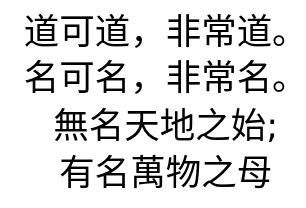
\includegraphics[scale=0.5]{./Images/Chinese.jpeg}
	\vspace{0.8cm} 

	\renewcommand{\corpsgrootte}{15pt}
\lol\pe\Atlanpi\tom\comma \Atlanne\si \lol\tet

\na\pe\Atlanpi\na\comma \Atlanne\si \na\tet 

\si\Atlanne\Atlanpi\na\comma \si \mi \ta\som\an\tem 

\si\Atlanpi\na\comma \si \Atlanfi\pet \ta\on\mus 
\restorecorps

	\vspace{0.8cm} 

The Path that can be trodden, 

is not the eternal Path. 

The Name that can be named, 

is not the eternal Name. 

Nameless, it is the Originator  

of heaven and earth 

Named, it is the Mother  

of ten thousand things. 
}


\vspace{0.3cm}


-{\it Dao De Jing, chapter 1}

\end{center}


\pagebreak

\noindent {\Large Foreword - by Ana Bosni\'{c}}

\noindent It is my distinct pleasure to write the foreword to this work by Stijn, Niek, Jarno, Jep, Jonathan and Max, students of the Humanities Honors Program at Utrecht University. As this book shows, they have attempted to create a new language (one with the potential for universal adoption), thus embarking on a linguistic adventure packed with challenges, curiosity, and a dash of audacity.  

Creating a new language is a complex, interdisciplinary task requiring skills, time, effort, dedication, motivation, endless creativity, and above all – (linguistic) knowledge. There also needs to be a deeper understanding of linguistic notions and theories, complexities that underpin human communication, the cultural diversity that influences our lexicon, and the paradox of simplicity and expressiveness.  

The authors have embarked on this journey to create Atlan, trying to develop a universal, neutral, and simple language; a language that should be able connect people, transcend boundaries, and be embraced by diverse communities. Ambitiously, they have attempted to craft a linguistic framework that would not favor any specific culture or group, but rather provide a neutral platform for human communication. Needless to say, that this was a titanic task, and the mere act of attempting it is praiseworthy.  

 As a constructed language, Atlan benefits from the kind of tools that an organically generated language cannot. Thus, for example, the creators of Atlan have tapped into vast reservoirs of linguistic data to inform their decisions, allowing them to create Atlan’s phonetic inventory, script and vocabulary. This fusion of human creativity and computational insights laid the foundation for their linguistic invention, offering a boost in their pursuit of universality, unambiguity, and parsimony. It goes without saying that this innovative approach to language creation serves as a testament to the boundless possibilities that arise when human creativity converges with computational tools.  

In conclusion, this book encapsulates the result of the arduous work carried out by Stijn, Niek, Jarno, Jep, Jonathan, and Max in their quest to create a universal and neutral auxiliary language. Throughout the pages of this book, readers will bear witness to their tireless pursuit to create a language that transcends borders and fosters effective global communication. It is my hope that their journey inspires further research into the intricacies of language, serves as a reminder that the power of human ingenuity knows no bounds, and shows that linguistics can be fun!  

And can Atlan become a new lingua franca? Well, only time will tell. 



\hfill Ana Bosni\'{c}
